%-----------------------------------------------------------------------
% Beginning of chap2.tex
%-----------------------------------------------------------------------
%
%%%%%%%%%%%%%%%%%%%%%%%%%%%%%%%%%%%%%%%%%%%%%%%%%%%%%%%%%%%%%%%%%%%%%%%%

\chapter[METHODS]{Methods} 
\section{Study Areas}
To address my research questions, I analyzed nine Texas coastal plain streams falling along a precipitation, and subsequently, a land use gradient (Figure~\ref{Fig:PPT}~and~\ref{Fig:LandUse}). I estimated ecosystem metabolism in these streams from continuous measurements of dissolved oxygen and temperature for the time periods of 2017-2018 and 2020-2021.

Watershed areas for each of the nine sites were delineated from 1/3 arc-second digital elevation models (DEM) from the United States Geological Survey (USGS). I then calculated watershed land usage percentages using the National Land Cover Data-set (NLCD, 2019). All GIS analysis took place in ArcMap (Version 10.8, ESRI, USA) and QGIS (Version 3.22, QGIS Development Team, Switzerland).

\section{Site Descriptions}
The annual average precipitation along the coastal plain ranged from 55 cm~yr$^{-1}$ in the semi-arid to 135 cm~yr$^{-1}$ at the most mesic watershed along the 300 km precipitation gradient \cite{PRISM}. The catchment areas of the streams ranged from 73 to 1787 \unit{\square\km} (Table \ref{tab:WS Area}). Sites are characterized with high turbidity and intact riparian zones, ranging from dense forested canopy areas at the most mesic site to tall grasses at the most arid site (Figure~\ref{Pic:WMC}~and~\ref{Pic:TRC}). While these sites had intact riparian zones, watershed land use varied across sites following the precipitation gradient, from semi-arid to mesic, agriculture land use increased from 33\% to 82\%, while non-agricultural vegetation decreased from 55\% to 1\% (Figure~\ref{Fig:LandUse}). The precipitation gradient likely drove land use. A majority of sites had sandy substrate that mobilized during precipitation events. Substrate at other sites was composed of small pebbles and gravel. 

\begin{figure}[htb]
\begin{center}
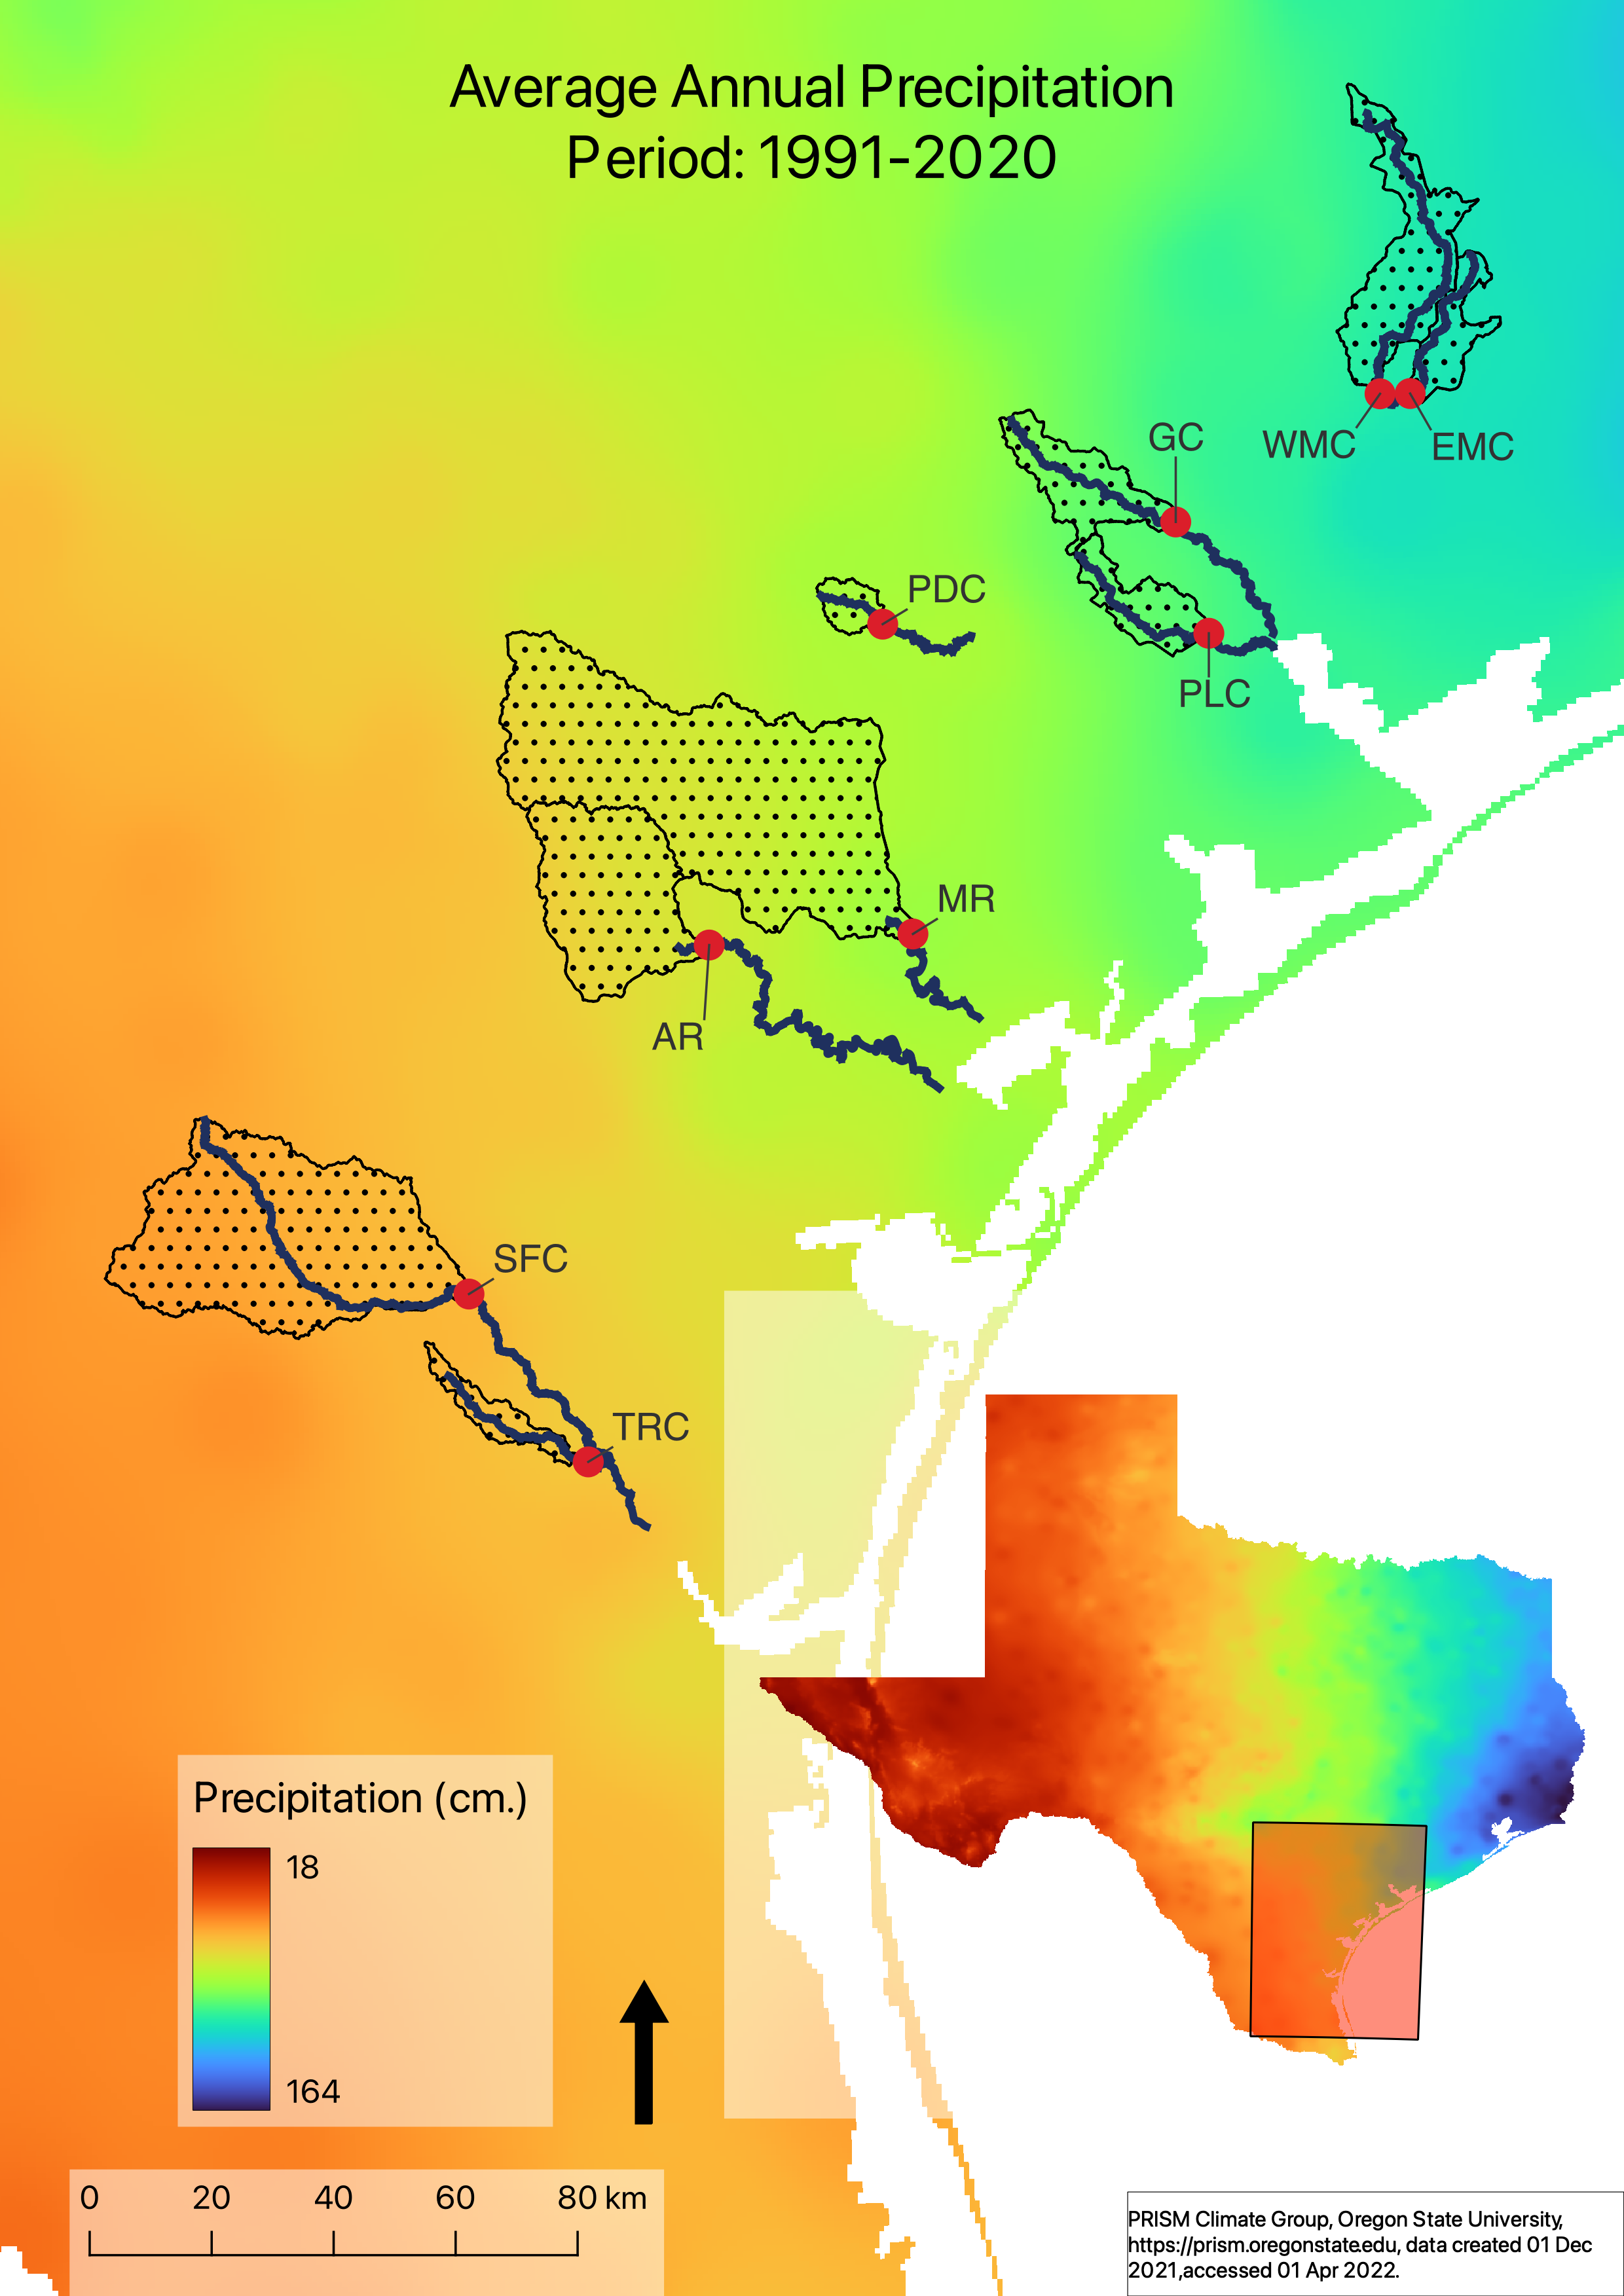
\includegraphics[scale = 0.7]{Figs/PPT.png}
\caption[Texas Precipitation Gradient]{\textit{Texas Precipitation Gradient.} The nine study sites and their watersheds across the 300 km coastal precipitation gradient.}
\label{Fig:PPT}
\end{center}
\end{figure}

\begin{landscape}
\begin{figure}[htb]
\begin{center}
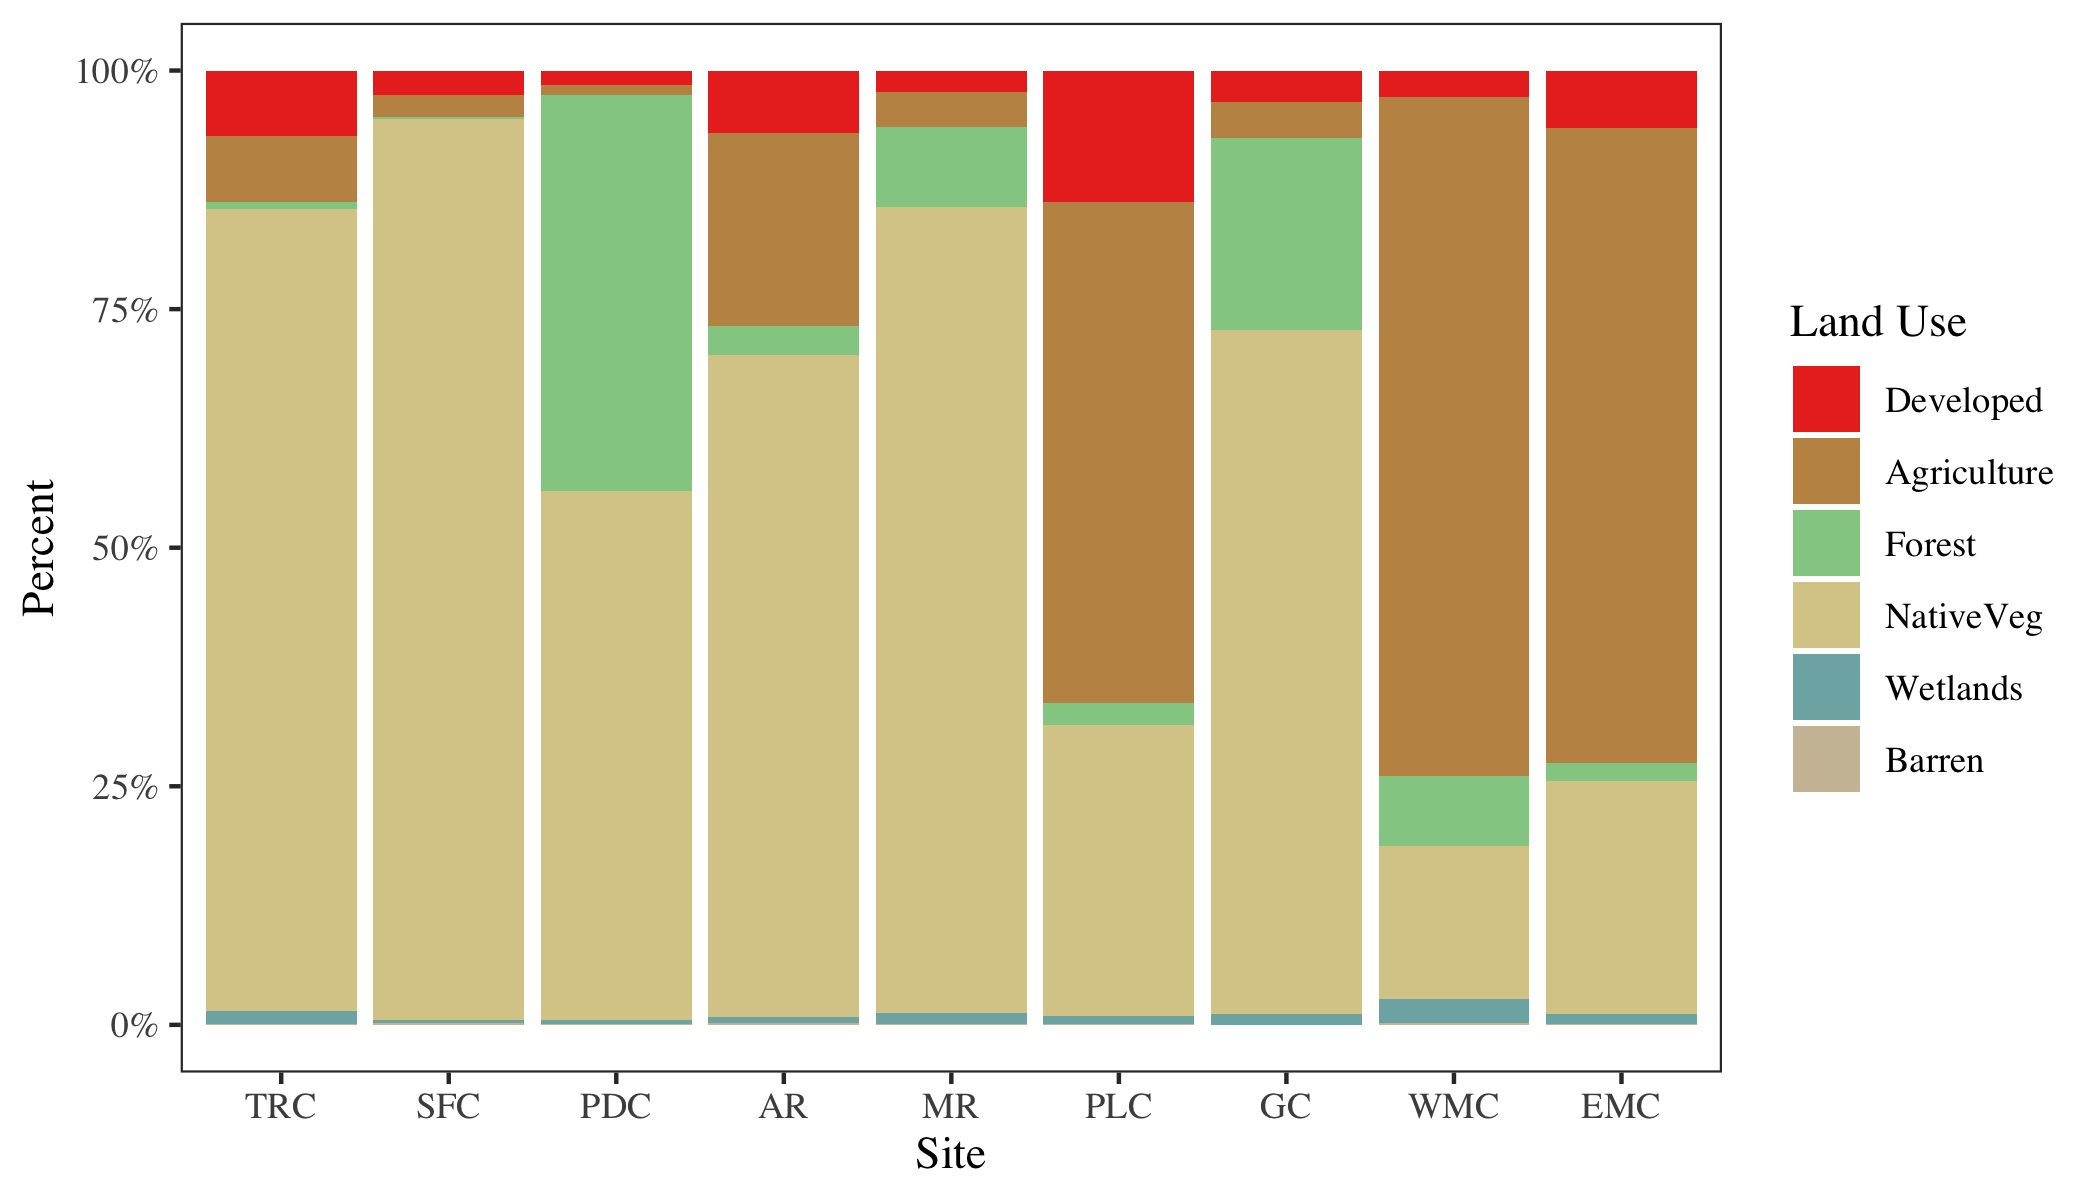
\includegraphics[scale=0.3]{Figs/LandUse.png}
\caption[Watershed Land Use]{\textit{Watershed Land Use.} Land cover types (\%) the nine study sites (Table \ref{tab:WS Area}). Sites are arranged from arid (left) to mesic (right).}
\label{Fig:LandUse}
\end{center}
\end{figure}
\end{landscape}

\begin{table}[htb]
\caption[Site Summary]{\textit{Site Summary}}
\begin{center}
\begin{tabular}
[c]{ccc}\hline
Site & Site Code & Watershed Area (\unit{\square\km})\\\hline
Tranquitas Creek & TRC & 126\\ 
San Fernando Creek & SFC & 1313\\ 
Aransas River & AR &  640 \\ 
Perdido Creek & PDC & 73 \\ 
Mission River & MR & 1787 \\ 
Placedo Creek& PLC & 177 \\ 
Garcitas Creek & GC & 273 \\ 
West Mustang Creek & WMC & 461\\ 
East Mustang Creek & EMC & 140\\\hline
\end{tabular}
\end{center}
\small \textit{Note}: Sites are arranged top to bottom, arid to mesic, with the site code. The largest watershed was 1787 \unit{\square\km}, while the smallest watershed was 73 \unit{\square\km}.
\label{tab:WS Area}
\end{table}

\begin{figure}[htb]
\begin{center}
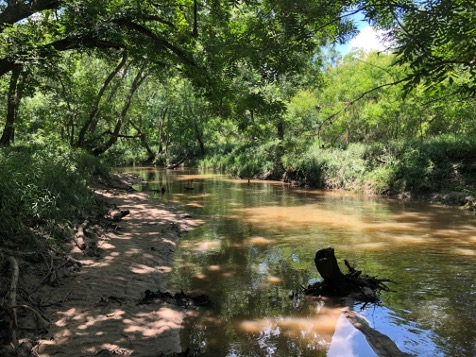
\includegraphics[scale = 0.8]{Figs/WMC.jpg}
\caption[WMC]{\textit{WMC.} This site is one of the most mesic sites and is characterized with high turbidity, high canopy cover, that likely decreases light availability, and sandy substrate.}
\label{Pic:WMC}
\end{center}
\end{figure}

\begin{figure}[htb]
\begin{center}
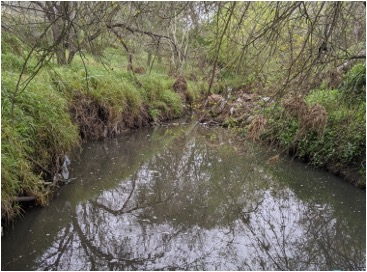
\includegraphics[scale = 0.8]{Figs/trc.jpg}
\caption[TRC]{\textit{TRC.} This site is the most arid site and is characterized with high turbidity and dense riparian vegetation, likely decreasing light availability.}
\label{Pic:TRC}
\end{center}
\end{figure}


\section{Ecosystem Metabolism}

I estimated daily GPP and ER from continuously measured dissolved oxygen concentrations using a one-station approach \cite{odum_primary_1956}. In one-station models, dissolved oxygen (DO) concentrations are used to estimate GPP, ER, and K$_O$ (gas exchange rate [\unit{\per\day}] for oxygen at stream water temperature). DO and temperature were measured every 10 minutes with miniDOT (PME) DO loggers in the stream thalweg, to ensure the water was well mixed. I used the R package StreamLight \cite{savoy_streamlight_2021}, this package uses NLDAS, LAI, and field measurements to estimate light for each site.  GPP, ER, and K$_O$ were modeled using the R package streamMetabolizer  \cite{appling_streammetabolizer_2018}. I used high frequency DO, temperature, and PAR to estimate GPP, ER, and K$_O$ using the following equation \cite{hotchkissHighRatesDaytime2014, hall_turbidity_2015, ulseth_climate-induced_2018, hall_gas_2019}:
\begin{equation*}\label{metab}
\text{O}_{i}=\text{O}_{i-\Delta t}+\left(\left(\frac{\text{GPP}_{d}}{\bar{Z}} \times \frac{\text{PAR}_{i}}{\sum \text{PAR}_{d}}\right)+\frac{\text{E R}_{d}}{\bar{Z}}+\text{K}_{o}\left(\text{O}_{{\text{sat}}(i-\Delta t)}-\text{O}_{i-\Delta t}\right)\right) \Delta t
\end{equation*}
Where O$_i$ is the DO (\unit{\mg\per\l}) concentration at time $i$ and and $O_{(i-\Delta t)}$ is the DO concentration at the time step prior to $O_i$ and $\Delta t$ is the time-step of the analysis (10 minutes). GPP$_d$ and ER$_d$ are areal fluxes of GPP and ER for day $d$ (\unit{\goxy}). $\bar{Z}$ is daily average stream reach depth (m). The gas exchange rate, K$_O$ is at stream water temperature. DO at saturation, O$_{sat}$ refers to oxygen concentration (\unit{\mg\per\l}) at 100\% saturation at stream water temperature and barometric pressure \cite{garcia_oxygen_1992}, which was measured at the Texas A\&M University—Corpus Christi Meteorological station (27° 42' 54" N, 97° 19' 43" W). PAR$_i$ (\unit{\umol} \unit{\per\square\m\per\s}) is photosynthetic active radiation at time $i$ calculated using a function in streamMetabolizer \cite{appling_streammetabolizer_2018} and $\sum$ PAR$_d$, is the light intensity for day $d$.


The Bayesian model from streamMetabolizer was used to estimate GPP, ER, and K$_{600}$, the gas exchange coefficient, normalized to normalized to a Schmidt number of 600. I used partial pooling of K$_{600}$ across all days from each site. The model was run for 2000 warm up steps and then 2000 saved steps, to ensure the Bayesian chains converge \cite{appling_metabolic_2018, arroita_twenty_2019}. The Baysian model was run with 4 chains, on 4 cores in parallel. 

I used several criteria to evaluate model fit. First, I used the relationship between ER and K$_{600}$, if ER and K$_{600}$ are strongly related the model did not fit, then days where K$_{600}$ exceeded 100 were thrown out, these are very high values and likely not plausible given the low slope and low turbulence of these coastal plain streams. Days with high stream flow (+ 2 SD) were also removed from the model, high stream flow results in a dilution of the diel oxygen signal, which becomes problematic when trying to estimate GPP, ER, and K$_{600}$. Additionally, when DO was equal to or less than 0.01 \unit{\mg\per\l}, these days were thrown out as this is when sensors were believed to be buried under sediment after large rain events. 


\section{DOC and Nutrients}
I collected water samples monthly to quantify nutrient (NO$_3$-N, NH$_4$-N, and PO$_4$-P) and DOC concentrations. I filtered water from each site with a \qty{0.7}{\um} pre-combusted glass fiber filter (GFF) into acid-washed 60 mL nalgene bottles for nutrients and acid-washed pre-combusted 40 mL glass vials for DOC for a total of 4 replicates for both nutrients and DOC. All samples were kept cold and in the dark until transported to the laboratory. Nutrient samples were frozen until analysis at Oklahoma State University Soil, Water and Forage Analytical Laboratory. DOC concentrations were measured using a Shimadzu TOC/TN analyzer at Sam Houston State University.  

\section{Discharge}
To characterize discharge and calculate average reach depth, field measurements of width, velocity, and gage measurements of discharge were retrieved from the United States Geological Survey. Using relationships of depth and discharge from each site, I calculated daily average stream depth, these measurements were then used as $\bar{Z}$, daily average stream reach depth (m), in the equation above \cite{dataRetrival, surveyUSGSWaterData1994, raymond_scaling_2012}

\section{Statistical Analysis}


To quantify the effect of land use and the precipitation gradient on ecosystem metabolism, I used structural equation modeling (SEM) to test my hypotheses (Figure~\ref{fig:concept}) \cite{bernot_inter-regional_2010, fus_land_2017}. SEMs are used when there is an underlying mechanism that is causing co-variance between random variables, it also take into account correlated independent variables, measurement error, and provides a more robust analysis compared to multivariate approaches \cite{malaeb_using_2000, bernot_inter-regional_2010}. To group land use categories for the structural equation model, I used a principal components analysis (PCA) \cite{rcore}. The two land use PCs were used in the structural equation model as a proxy for land use. I included log-transformed monthly estimates of GPP, ER, DOC concentration, and turbidity, monthly averages of NO$_3$-N, PO$_4$-P, precipitation, and discharge. I used Standardized Root Mean Square Residual (SRMR) to compare model fit. Statistical analysis was preformed with R version 4.1.0 and lavaan \cite{rcore, rosseel_lavaan}.

\endinput

%-----------------------------------------------------------------------
% End of chap2.tex
%-----------------------------------------------------------------------
